This chapter will finally compare Aparapi and JCuda based on the test battery we applied on them in the previous chapter.

As discussed in the introduction (see section \ref{goals}), our comparison is based on the execution speed and ease of use. We will discuss each comparison point for Aparapi and JCuda so as to evaluate which one is better for each criteria.

The next chapter will be an overall conclusion, bringing the final thoughts and perspectives.

\section{Execution speed}

For the execution speed, two benchmarks were used and executed against Aparapi and JCuda. The baseline used for the speedup were a native execution on a vanilla Java code using only the host's CPU.

Each benchmark is testing a different type of computation. The matrix multiplication is more focused on floating point operations while the Levenshtein distance is more focused on char operations.

For each benchmark, we will compare the speedup gained using Aparapi and JCuda.

\subsection{Matrix}

The following table is a side by side comparison of Aparapi and JCuda for the matrix multiplication, based on the speedup.

\renewcommand{\arraystretch}{2}
\begin{figure}[H]
\begin{tabular}[width=1\textwidth]{c|c}
	\textbf{Aparapi} & \textbf{JCuda} \\
	\hline \hline
	\multicolumn{2}{c}{Speedup plot} \\
	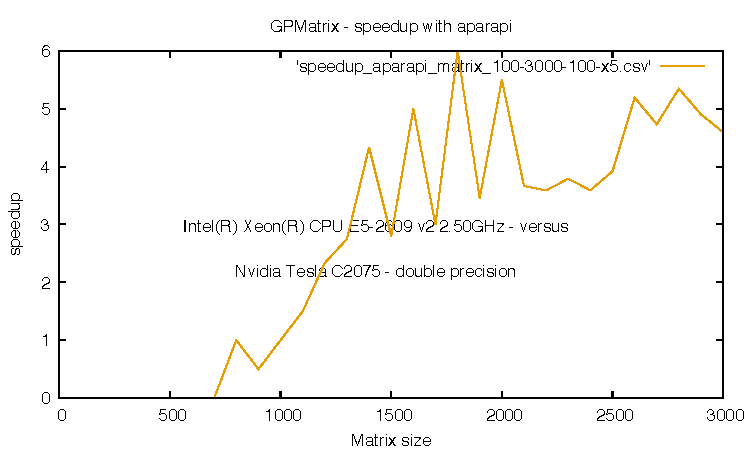
\includegraphics[width=.5\textwidth]{speedup_aparapi_matrix_5x.pdf} &
	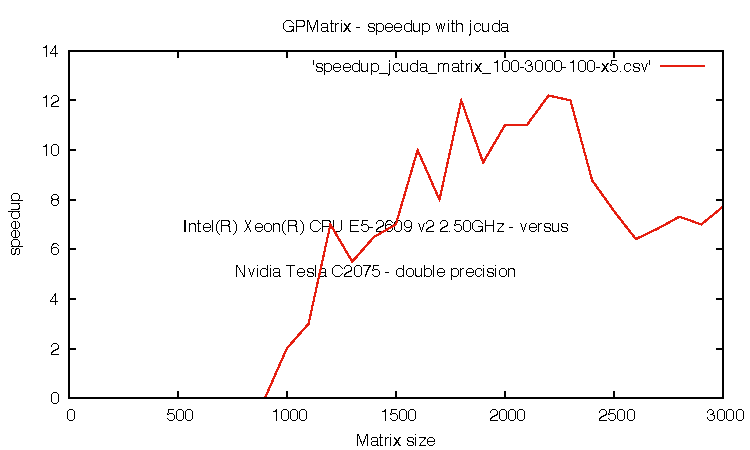
\includegraphics[width=.5\textwidth]{speedup_jcuda_matrix_5x.pdf} \\
	\hline
	\multicolumn{2}{c}{Speedup peak} \\
	\textcolor{BrickRed}{6} & \textcolor{OliveGreen}{\textbf{12.2}} \\
	\hline
	\multicolumn{2}{c}{Speedup average} \\
	\textcolor{BrickRed}{2.3} & \textcolor{OliveGreen}{\textbf{5.6}} \\
	\hline
	\multicolumn{2}{c}{Speedup median} \\
	\textcolor{BrickRed}{3.4} & \textcolor{OliveGreen}{\textbf{7}} \\
	\hline
	
\end{tabular}
\end{figure}

On this turn, JCuda shows a clear better performance on all the metrics, having globally an execution time 2 times faster than Aparapi. But it is worth noting that JCuda seems to suddenly decrease performance after a certain matrix size (around 2400), while Aparapi show a globally more stable speedup. But even with this consideration, JCuda always shows a better speedp.

\subsection{Levenshtein}

The following table is a side by side comparison of Aparapi and JCuda for the Levenstein distance computation, based on the speedup.

\begin{figure}[H]
\begin{tabular}[width=1\textwidth]{c|c}
	\textbf{Aparapi} & \textbf{JCuda} \\
	\hline \hline
	\multicolumn{2}{c}{Speedup plot} \\
	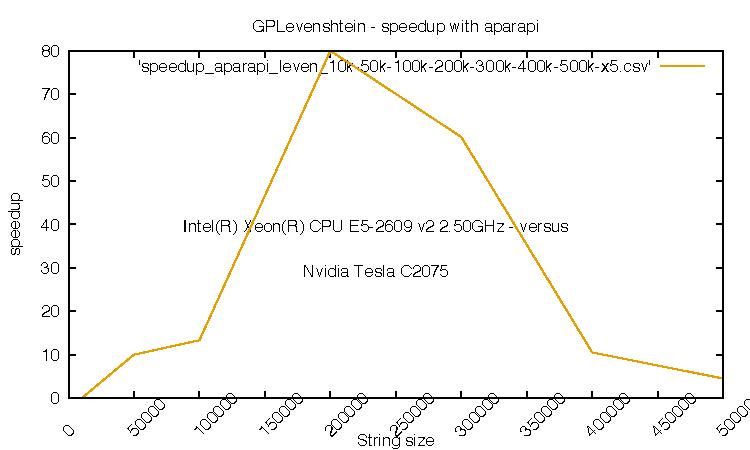
\includegraphics[width=.5\textwidth]{speedup_aparapi_leven_5x.pdf} &
	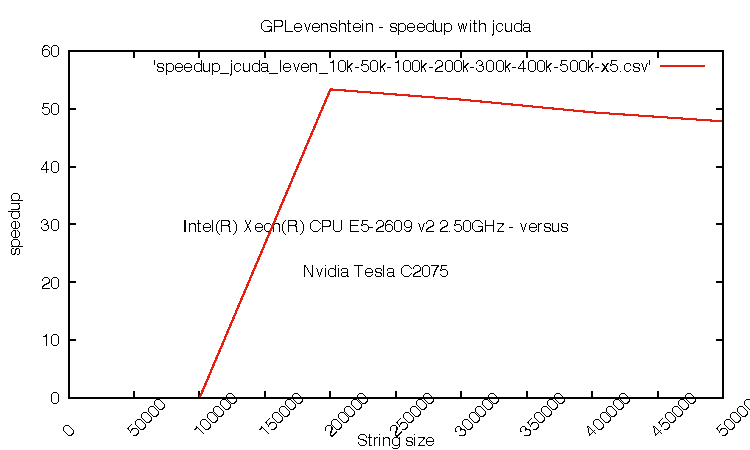
\includegraphics[width=.5\textwidth]{speedup_jcuda_leven_5x.pdf} \\
	\hline
	\multicolumn{2}{c}{Speedup peak} \\
	\textcolor{OliveGreen}{\textbf{80}} & \textcolor{BrickRed}{53.3} \\
	\hline
	\multicolumn{2}{c}{Speedup average} \\
	\textcolor{BrickRed}{25.2} & \textcolor{OliveGreen}{\textbf{28.5}} \\
	\hline
	\multicolumn{2}{c}{Speedup median} \\
	\textcolor{BrickRed}{10} & \textcolor{OliveGreen}{\textbf{47.8}} \\
	\hline
	
\end{tabular}
\end{figure}

Unlike with the matrix multiplication, this time we can't clearly define which solution is faster. Aparapi is globally less fast than JCuda but has the best peak with up to 80 times faster compared with JCuda - who has up to 53.3 times faster. The only answer we can give is "it depends". Around a string size of 200k, Aparapi is better than JCuda. But as soon as we have a bigger string size (around 300k), JCuda is a faster solution and shows a more stable speedup with an increasing string size. Based on the average speedup, JCuda is globally faster.

\section{Ease of use}

To evaluate the ease of use, we will be looking at the following aspects:
\begin{enumerate}
  \item The installation process
  \item The number of code lines
  \item The external feedbacks
  \item The problems encountered and restrictions
\end{enumerate}

\subsection{Installation process}

In both cases - with Aparapi and JCuda - the installation process were very similar and fast. Despite the fact that we didn't have any difficulties getting started and installing both of the solutions, we give the medal to JCuda for this turn.

JCuda was easier to instal due to a better documentation, providing examples and command lines to compile and execute a JCuda based program. This support wasn't as good with Aparapi, where we didn't really find any good getting started explanation.

\subsection{Line of codes}

The following table is a side by side comparison of Aparapi and JCuda concerning the line of codes needed to run the matrix multiplication and Levenshtein distance computation. In parenthesis are the differences with the number of code lines for the vanilla Java implementation.

\newcolumntype{Y}{>{\centering\arraybackslash}X}
\begin{figure}[H]
\begin{tabularx}{\textwidth}{@{}Y|Y|Y@{}}
	\textbf{Aparapi} & \textbf{JCuda} & \textbf{(Vanilla)} \\
	\hline \hline
	\multicolumn{3}{c}{Matrix multiplication} \\
	\textcolor{OliveGreen}{\textbf{21} (+8)} & \textcolor{BrickRed}{47 (+34)} & 13 \\
	\hline
	\multicolumn{3}{c}{Levenstein distance computation} \\
	\textcolor{OliveGreen}{\textbf{24} (+6)} & \textcolor{BrickRed}{51 (+38)} & 18 \\
	\hline
	
\end{tabularx}
\end{figure}

Aparapi wins by far this turn with more than 2 times less lines of code needed to perform the same task than with JCuda.

Aparapi was much easier to implement in terms of code lines needed. This difference with JCuda is mainly due to the need for JCuda to set each kernel attribute so it is available to the kernel method - which is written in C. This process requires many steps. For a quick use, Aparapi is more suitable than JCuda.

\subsection{External feedback}

The following table summarizes the external feedback on how developers evaluated the difficulty to understand the code - especially the part performing computation on the GPU. They had to give a mark from 1 (very difficult) to 5 (very easy). In the following table are the averages' marks.

\newcolumntype{Y}{>{\centering\arraybackslash}X}
\begin{figure}[H]
\begin{tabularx}{\textwidth}{@{}Y|Y|Y@{}}
	\textbf{Aparapi} & \textbf{JCuda} \\
	\hline \hline
	\multicolumn{2}{c}{Matrix multiplication - external developers feedback average marks} \\
	\textcolor{OliveGreen}{\textbf{5}} & \textcolor{BrickRed}{3.5} \\
	\hline
	\multicolumn{2}{c}{Levenstein distance - external developers average feedback marks} \\
	\textcolor{OliveGreen}{\textbf{5}} & \textcolor{BrickRed}{3.5} \\
	\hline
	
\end{tabularx}
\end{figure}

Aparapi seems to be more easier to understand than JCuda. It is probably due to the fact that JCuda requires more lines of code and a kernel written in C. The external feedback were performed with 2 developers having already an experience in GPU programming.

\subsection{Problems encountered - restrictions}

\begin{figure}[H]
\begin{tabularx}{\textwidth}{@{}Y|Y@{}}
	\textbf{Aparapi} & \textbf{JCuda} \\
	\hline \hline
	 
	 \begin{itemize}
	   \item
	   No official getting started guide found. We had to use examples so as to start using Aparapi.
       \item 
       Impossible to use any Java objects inside the kernel method. We had to write our own min() methods and convert strings to char arrays. 
       \item
       Impossible to get the size of an array inside the kernel. It is a known issue \cite{aparapibug}.
     \end{itemize} 
     
     &

	 \begin{itemize}
       \item Like Aparapi, impossible to use Java objects but even any Java code inside the kernel method.
       \item The kernel method is written in C, not in Java. This restricts the use of Java but makes the reusability and sharing of existing CUDA kernel methods possible.
       \item Impossible to write a simple min() method for the kernel, making the code hard to read.
     \end{itemize} \\

	\hline
	
\end{tabularx}
\end{figure}
\renewcommand{\arraystretch}{1}

In terms of restrictions, we can't clearly give a single medal to Aparapi or JCuda. The answer is "it depends". Either Aparapi or JCuda can't use Java objects in the kernel methods. Aparapi has the advantage of being fully usable under a Java workflow, while JCuda needs a kernel written in C. Aparapi gives the ability to have custom methods available from the kernel, giving more flexibility. On the other hand, JCuda has it's kernel written in C, giving the ability to use already written CUDA kernel methods. This also makes the use of JCuda from someone already knowing CUDA easy, since the kernel code remains the same, and the process, for JCuda, of calling the kernel method is also very similar as one we would do with vanilla CUDA programming.

For someone already knowing CUDA, JCuda gives a better way to use the GPU from a Java code. But this only under a CUDA compatible environment.

For someone looking for a full Java solution to write GPU code, having an OpenCL environement and giving the ability to write flexible methods available from the kernel, Aparapi is a better solution.